%%%%%%%%%%%% Attribution %%%%%%%%%%%%
% This template was created by 
% Chuck F. Rocca at WCSU and may be
% copied and used freely for 
% non-commercial purposes.
% 10-17-2021
%%%%%%%%%%%%%%%%%%%%%%%%%%%%%%%%%%%%%

%%%%%%% Start Document Header %%%%%%%
% In creating a new document
% copy and paste the header 
% as is.
%%%%%%%%%%%%%%%%%%%%%%%%%%%%%%%%%%%%%

\documentclass[12pt]{article}

%%%% Header Information %%%%
    \include{header}

%%%% Document Information %%%%
    \title{Homework Template and Samples}
    \author{Ford Prefect}
    \date{October \(12^{th}\) 1979}

%%%%%%% End Document Header %%%%%%%


%%%% Begin Document %%%%
% note that the document starts with
% \begin{document} and ends with
% \end{document}
%%%%%%%%%%%%%%%%%%%%%%%%

\begin{document}

%%%% Format Running Header %%%%%
\markboth{\theauthor}{\thetitle}

%%%% Insert the Title Information %%%
\maketitle


%%%% General Description of the Document %%%%
\begin{abstract}
    This document introduces a standard template box for typing up homework.  This can help make homework look better and be easier to read. The suggested template box also automatically leaves a space for an instructor to leave comments and insert a grade.
\end{abstract}


%%%% Introduction to the General Template %%%%
\section{The Template}

Here is a blank Template Box:
    \begin{problem}{Title Goes Here}
        Answer Goes Here!!!
    \end{problem}

\noindent
The code for this in the \LaTeX\ document looks like this:
    \begin{minted}{latex}
        \begin{problem}{Title Goes Here}
            Answer Goes Here!!!
        \end{problem}
    \end{minted}

\noindent
Whenever you want to type up a new problem you insert the above code, change the title to give the page and problem number, and type the solution in between the begin and end tags (where it says answer goes here).  This way multiple questions might look like this:
    \begin{problem}{p.xyz \# 23}
        Answer Goes Here!!!
    \end{problem}
    \begin{problem}{p.yzx \# 32}
        Answer Goes Here!!!
    \end{problem}
    \begin{problem}{p.zxy \# 5}
        Answer Goes Here!!!
    \end{problem}

\noindent
And since they are all typed up it is easier to rearrange them or edit them.

\noindent
In the following section there are a set of increasingly intricate examples of problems including the necessary code to type them up.  You can of course also look at the raw code.

%%%% Examples of Typed Up Problems %%%%
\section{Sample Problems}

%%%% Equations %%%%
% Examples of inline,
% displayed, and stacked
% equations.
%%%%%%%%%%%%%%%%%%%

\begin{problem}{p.42 \# 1952: Some Equations}
    In this exercise we demonstrate an inline expression like\\ \(f(x)=x^2-4x=4\), which is typeset like so \mintinline{latex}{\(f(x)=x^2-4x=4\)} and in solving $f(x)=0$ we can demonstrate a displayed equation as well:
        \[f(x)=0\Rightarrow x^2-4x+4=(x-2)^2=0 \Rightarrow x=2,\]
    which is typed like so:
    
\begin{center}
\mintinline{latex}{
\[f(x)=0\Rightarrow x^2-4x+4=(x-2)^2=0 \Rightarrow x=2,\]
}
\end{center}
    
    Or, better yet with a stacked equation:
    \begin{align}
    % Line 1
        f(x) = 0 
    % note that the & tells LaTeX where to line things up
    % the \\ tells LaTeX to start a new line
            &\Rightarrow x^2-4x+4=0 \\
    % Line 2
            &\Rightarrow (x-2)^2=0\\
    % Line 3
            &\Rightarrow x-2=0\\
    % Line 4
            &\Rightarrow x=2,
    \end{align}
    which is typed as

\begin{minted}{latex}
\begin{align}
% Line 1
    f(x) = 0 
% note that the & tells LaTeX where to line things up
% the \\ tells LaTeX to start a new line
        &\Rightarrow x^2-4x+4=0 \\
% Line 2
        &\Rightarrow (x-2)^2=0\\
% Line 3
        &\Rightarrow x-2=0\\
% Line 4
        &\Rightarrow x=2,
\end{align}
\end{minted}

\end{problem}




%%%% Table %%%%
% An array used to create
% a truth table, also shows some
% logic symbols.
%%%%%%%%%%%%%%%

\begin{problem}{p.314 \# 159: A Truth Table}
    To demonstrate that the following is true 
    \[P\rightarrow Q\equiv \sim (P\wedge \sim Q)\equiv \sim P\vee Q\]
    we can use this truth table
    \[
        % |*{8}{c|} gives 8 columns with 
        % centered text in each
        \begin{array}{|*{8}{c|}}
        % header row
        % similar to align, & indicates a 
        % new column and \\ ends a row
            P & Q & \sim P & \sim Q 
                &  P \rightarrow Q 
                & P\wedge \sim Q
                & \sim(P\wedge \sim Q)
                & \sim P\vee Q\\ \hline
        % row 1
            T & T & F & F & T & F & T & T \\
        % row 2
            T & F & F & T & F & T & F & F \\
        % row 3
            F & T & T & F & T & F & T & T \\
        % row 4
            F & F & T & T & T & F & T &  T \\
        \end{array}
    \]
    which is typeset using this code

\begin{minted}{latex}
\[
    % |*{8}{c|} gives 8 columns with 
    % centered text in each
    \begin{array}{|*{8}{c|}}
    % header row
    % similar to align, & indicates a 
    % new column and \\ ends a row
        P & Q & \sim P & \sim Q 
            &  P \rightarrow Q 
            & P\wedge \sim Q
            & \sim(P\wedge \sim Q)
            & \sim P\vee Q\\ \hline
    % row 1
        T & T & F & F & T & F & T & T \\
    % row 2
        T & F & F & T & F & T & F & F \\
    % row 3
        F & T & T & F & T & F & T & T \\
    % row 4
        F & F & T & T & T & F & T &  T \\
    \end{array}
\]
\end{minted}

\end{problem}



%%%% Tall Delimiters and Sets %%%%
% Demonstration of taller delimiters,
% i.e. (), {}, ||, etc. and some set
% operations.
%%%%%%%%%%%%%%%%%%%%%%%%%%%%%%%%%%

\begin{problem}{p.271 \# 8e: Some Set Stuff}
    If \(A=\{1,a,\alpha\}\), then
    \[
        \left|\mathscr{P}(A)\right|=\left|\left\{
            \emptyset, \{1\},\{a\},\{\alpha\},
            \{1,a\},\{1,\alpha\},
            \{a,\alpha\},\{1,a,\alpha\}
        \right\}\right|=8.
    \]
    If we now let $B=A\cup \{2\}$ then
    \begin{align}
    % row 1
        \left|\mathscr{P}(B)\right| 
            &=\left|\mathscr{P}(A)\cup\left(
                \bigcup_{S\in\mathscr{P}(A)}\{S\cup \{2\}\}
            \right)\right| \\
    % row 2
            &=\left|\mathscr{P}(A)\right|+\left|\left(
                \bigcup_{S\in\mathscr{P}(A)}\{S\cup \{2\}\}
            \right)\right| \\
    % row 2
            &=\left|\mathscr{P}(A)\right|
            +\left|\mathscr{P}(A)\right| \\
    % row 4
            &= 8+8\\
    % row 5
            &= 16
    \end{align}
    The above was typeset as follows:
    
\begin{minted}{latex}
\begin{align}
% row 1
    \left|\mathscr{P}(B)\right| 
        &=\left|\mathscr{P}(A)\cup\left(
            \bigcup_{S\in\mathscr{P}(A)}\{S\cup \{2\}\}
        \right)\right| \\
% row 2
        &=\left|\mathscr{P}(A)\right|+\left|\left(
            \bigcup_{S\in\mathscr{P}(A)}\{S\cup \{2\}\}
        \right)\right| \\
% row 2
        &=\left|\mathscr{P}(A)\right|
        +\left|\mathscr{P}(A)\right| \\
% row 4
        &= 8+8\\
% row 5
        &= 16
\end{align}
\end{minted}

    \noindent
    Note in particular the use of \mintinline{latex}{\left( ... \right)} to make really tall delimiters.
\end{problem}


%%%%% Including an Image %%%%%
% Here is an example of 
% including an uploaded 
% image.
%%%%%%%%%%%%%%%%%%%%%%%%%%%%%%

\begin{problem}{p.667 \# 10\, e-13: Some Scrap Work}
    Here is a picture of scrap work for a problem from linear algebra:
        \begin{center}
            \includegraphics[width=0.75\textwidth]{Linear_Scrap.png}
        \end{center}
    The code for including this, once it is uploaded, is:
    
\begin{minted}{latex}
\includegraphics[width=0.75\textwidth]{Linear_Scrap.png}
\end{minted}
\end{problem}


%%%%% Adding in a diagram %%%%
% Here are some more expressions,
% and an example of including a 
% relatively basic diagram.
%%%%%%%%%%%%%%%%%%%%%%%%%%%%%%

\begin{problem}{p.662 \# 10\, e-36: Some Relations}
    Define a relation from a set \(A=\{1,2,3\}\) to itself by
        \[a\, R\, b:a\leq b\]
    The ordered pairs in this relation are
        \[R=\{(1,1),(1,2),(1,3),(2,2),(2,3),(3,3)\}\]
    which we can represent as a digraph by
    \begin{center}
        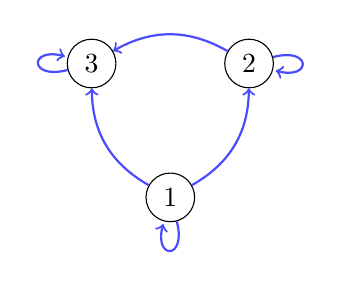
\begin{tikzpicture}
        %%%% Add nodes for each number
            \node[shape=circle,draw] (1) at (0,0) {1};
            \node[shape=circle,draw] (2) at (1,1.7) {2};
            \node[shape=circle,draw] (3) at (-1,1.7) {3};
        %%%% Add edges between nodes
            \draw[->,color=blue!70,thick] (1) to[bend right] (2);
            \draw[->,color=blue!70,thick] (1) to[bend left] (3);
            \draw[->,color=blue!70,thick] (2) to[bend right] (3);
        %%%% Add self referential edges 
            \draw[->,color=blue!70,thick] (1) edge[loop below] (1);
            \draw[->,color=blue!70,thick] (2) edge[loop right] (2);
            \draw[->,color=blue!70,thick] (3) edge[loop left] (3);
        \end{tikzpicture}
    \end{center}
    which was drawn with the code:
\begin{minted}{latex}
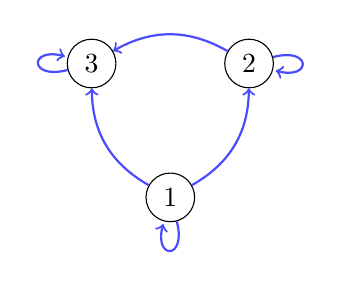
\begin{tikzpicture}
%%%% Add nodes for each number
    \node[shape=circle,draw] (1) at (0,0) {1};
    \node[shape=circle,draw] (2) at (1,1.7) {2};
    \node[shape=circle,draw] (3) at (-1,1.7) {3};
%%%% Add edges between nodes
    \draw[->,color=blue!70,thick] (1) to[bend right] (2);
    \draw[->,color=blue!70,thick] (1) to[bend left] (3);
    \draw[->,color=blue!70,thick] (2) to[bend right] (3);
%%%% Add self referential edges 
    \draw[->,color=blue!70,thick] (1) edge[loop below] (1);
    \draw[->,color=blue!70,thick] (2) edge[loop right] (2);
    \draw[->,color=blue!70,thick] (3) edge[loop left] (3);
\end{tikzpicture}
\end{minted}

\end{problem}

\end{document}
